%! Author = mr
%! Date = 8/8/2025

% Preamble
\documentclass[11pt]{article}

% Packages
\usepackage{amsmath}
\usepackage{tikz}
\usepackage[utf8]{inputenc}
\usepackage[T1]{fontenc}

\begin{document}

\section*{Abstract}

In this work, I explore time dilation within a three-dimensional superfluid Æther framework, where gravity and relativistic effects emerge from the internal motion of the Æther itself. The model treats the Æther as a compressible, inviscid medium threaded with vortex cores, whose rotation and flow patterns influence local time rates. By examining the geometry and energetics of these swirling structures, I show how classical gravitational time dilation can arise without invoking spacetime curvature. The discussion bridges well-known relativistic formulas with the mechanics of vortex motion, and proposes experimental conditions—realistic in principle—under which such effects might be detected in a laboratory. While speculative, the approach aims to link familiar relativistic predictions to an underlying fluid-dynamic mechanism.

\section*{Introduction}

Time dilation is usually presented as a geometric effect: clocks tick differently because spacetime is curved, or because an observer is in relative motion. That is the language of General Relativity and Special Relativity, and it works remarkably well. But I found myself wondering—what if there’s something physically tangible underneath that geometry? What if the passage of time is tied to the motion of a medium we can, at least in theory, model directly?

The starting point here is the superfluid Æther picture: a continuous, frictionless medium filling all of space, capable of supporting vortices much like those in liquid helium or Bose–Einstein condensates. In this setting, the “gravitational potential” is not a mysterious metric term but a property of swirl: the kinetic and rotational energy stored in the flow. If the flow is fast enough, local processes slow down—clocks tick differently—not because space is warped, but because the medium that carries all interactions is in motion.

In the following sections, I set out the core assumptions of the model, walk through the derivation of the time-dilation formula from the swirl velocity field, and compare the result to the standard Schwarzschild prediction. Along the way, I highlight similarities to, and differences from, other fluid-based analogies to gravity, and note where the Æther-based view may offer a more mechanical intuition.

\section*{2. Core Assumptions of the 3D Superfluid Æther Model}

To make any meaningful prediction, the model has to start with a set of assumptions. These are not arbitrary — they are chosen because they make the mathematics tractable and because they capture the physical picture I’m trying to test.

\begin{enumerate}
    \item The Æther as a Medium

    I treat the Æther as a continuous, inviscid (frictionless) fluid with a density $\rho_{\text{\ae}}$. In this view, space is not empty — it is filled with this medium, and every physical field is, in some sense, a pattern in it. While this is heresy to modern orthodoxy, it allows us to talk about time dilation as a mechanical effect, not just a geometric one.

    \item Vorticity as the Engine of Time Dilation

    In a rotating superfluid, a vortex line carries angular velocity $\boldsymbol{\omega}$. A point in the medium at radius $\mathbf{r}$ from the vortex core moves with tangential velocity
    \[
    \mathbf{v}_\theta = \boldsymbol{\omega} \times \mathbf{r}.
    \]
    In my hypothesis, this rotational motion is not just a byproduct — it directly affects the local ticking rate of clocks.

    \item Proper Time Relation

    Borrowing the structure from special relativity but giving it a fluid-dynamic origin, the proper time $\tau$ experienced by a “clock” moving with the medium satisfies
    \[
    \frac{d\tau}{dN} = \sqrt{ 1 - \frac{|\mathbf{v}_\theta|^2}{c^2} },
    \]
    where $N$ is the universal Æther time and $c$ is the signal propagation speed in the medium. This is the key link between swirl velocity and relativistic slowing.

    \item Stationary Flow for Simplicity

    The results here are derived for steady vortices — no turbulent bursts or time-varying flow. That’s a deliberate simplification, because turbulence would require a different mathematical treatment and might obscure the core mechanism.
\end{enumerate}

This section essentially defines the playing field. We now have a medium, a swirl velocity field, and a direct connection between that swirl and the rate at which time passes locally. The next step is to see how this gives rise to time dilation effects that look, numerically, just like those from relativity — even though the cause, in this model, is completely different.

\section*{3. Derivation of the Swirl-Induced Time Dilation Law}

Let’s start from something familiar: in special relativity, time dilation arises because a moving clock’s worldline through spacetime is “tilted” relative to a stationary one. In this Æther model, the picture is simpler — but stranger. Time slows down because the medium carrying all processes is itself in motion.

\subsection*{3.1 Geometry of the Flow}

Imagine a straight vortex line running along the $z$-axis in a superfluid. The flow is purely tangential in cylindrical coordinates $(r, \theta, z)$. At radius $r$, the swirl velocity is given by
\[
v_\theta = |\boldsymbol{\omega}| \, r,
\]
where $|\boldsymbol{\omega}|$ is the constant angular speed of the flow.

That’s the mechanical setup. No curvature, no exotic geometry — just a rotating medium.

\subsection*{3.2 Linking Swirl to Proper Time}

The core postulate of this model is that the ticking rate of a clock carried along by the Æther is reduced according to
\[
\frac{d\tau}{dN} = \sqrt{1 - \frac{v_\theta^2}{c^2}},
\]
with $N$ as the universal Æther time. Substituting the velocity relation gives:
\[
\frac{d\tau}{dN} = \sqrt{1 - \frac{\omega^2 r^2}{c^2}}.
\]

This is exactly the same mathematical form as the Lorentz factor $\gamma^{-1}(v)$ from special relativity — but here the velocity $v$ is not motion through space; it is the rotational motion of the local medium.

\subsection*{3.3 The Laboratory Thought Experiment}

Picture a small, ultra-precise clock suspended at a fixed radius $r$ from the vortex core. From the clock’s own perspective, it’s stationary — but in reality, it’s embedded in a swirling medium. An observer in the Æther rest frame would see its processes slow down according to the above factor.

In principle, one could test this by creating a Bose–Einstein condensate with a single, stable vortex and placing a “clock” — some periodic process — in the flow. The model predicts that the clock would run slower the closer it is to the core.

\section*{4. Extending to a 3D Swirl Field}

Up to now, I’ve kept things deliberately simple: a single straight vortex, constant angular velocity, perfectly steady flow. That’s a good sandbox, but nature is rarely so tidy. If the Æther really behaves like a superfluid, vortices will bend, merge, and form more complex patterns — and the time-dilation law needs to survive in that more general setting.

\subsection*{4.1 From Cylinders to Curves}

Let’s replace the straight vortex line with a curved vortex filament. At any point along the filament, the local angular velocity vector $\boldsymbol{\omega}(\mathbf{x})$ can point in different directions. The tangential velocity field now takes the form:
\[
\mathbf{v}_\theta(\mathbf{x}) = \boldsymbol{\omega}(\mathbf{x}) \times \mathbf{r}_\perp,
\]
where $\mathbf{r}_\perp$ is the perpendicular distance from the vortex core at that point.

The basic rule doesn’t change: the faster the swirl at a location, the slower the proper time there ticks relative to universal Æther time.

\subsection*{4.2 Generalized Time Dilation Formula}

For an arbitrary 3D swirl field, the dilation factor becomes:
\[
\frac{d\tau}{dN} = \sqrt{1 - \frac{|\mathbf{v}_\theta(\mathbf{x})|^2}{c^2}}.
\]
In principle, this is valid for any smooth velocity field that can be decomposed into vortex components.

This makes the model flexible: you can feed in a complex fluid-dynamics solution, and out comes a time-dilation map — no spacetime metric needed.

\subsection*{4.3 The Gravitational Analogy}

Here’s where the analogy sharpens. In general relativity, gravitational time dilation near a massive body comes from the curvature of spacetime, encoded in the metric tensor $g_{\mu\nu}$. In the vortex Æther picture, the same slowing emerges from the kinetic energy density of the swirling medium:
\[
U_\text{vortex} = \frac{1}{2} \rho_{\text{\ae}} |\boldsymbol{\omega}|^2.
\]
Regions of high rotational energy behave like regions of high gravitational potential in the relativistic picture.

If that correspondence holds — and that’s the big “if” — then gravity could be reinterpreted not as geometry, but as the emergent effect of coherent swirl patterns in a deeper substrate.

\section*{5. Comparison with Schwarzschild Time Dilation}

The Schwarzschild solution to Einstein’s field equations gives the time dilation for a stationary observer at radius $r$ from a spherical mass $M$:
\[
\frac{d\tau}{dt} = \sqrt{1 - \frac{2GM}{rc^2}}.
\]
It’s clean, it’s precise, and it has passed every experimental test we’ve thrown at it so far.

The question is: can the vortex Æther model produce a formula that matches this — not in spirit, but in actual numbers?

\subsection*{5.1 Matching the Functional Form}

In the Æther picture, we already have:
\[
\frac{d\tau}{dN} = \sqrt{1 - \frac{v_\theta^2}{c^2}}.
\]
If we want this to match the Schwarzschild factor, we can set:
\[
v_\theta^2 = \frac{2GM}{r}.
\]
That’s an interesting bridge: the swirl velocity at radius $r$ plays the role of the escape velocity in Newtonian gravity. In other words, where general relativity talks about spacetime curvature, the Æther model talks about the local speed of the medium — and the math lines up.

\subsection*{5.2 Interpretation}

If this mapping is valid, then the mass $M$ is not “bending spacetime” in the geometric sense. Instead, it’s stirring the Æther into a rotational pattern whose speed profile matches what we would otherwise call the gravitational potential. The deeper you go into the vortex — the smaller $r$ becomes — the faster the swirl, and the slower your clock ticks.

\subsection*{5.3 Limitations}

Of course, there’s a catch. The Schwarzschild metric also predicts spatial curvature, light bending, and other effects that this basic swirl model doesn’t yet account for. Matching time dilation is an encouraging start, but it’s only one piece of the puzzle. Without the rest, the Æther model is more of a shadow of gravity than a full replacement.

\section{Time Dilation in Hydrogen Atoms within the Vortex Æther Model}

In the Vortex Æther Model (VAM), space is permeated by an inviscid, superfluid medium --- the Æther --- which supports topological excitations in the form of knotted field structures. In the hydrogen atom, the proton consists of three quarks, each represented as either a $6_4$ (up) or $6_1$ (down) Fourier-series knot in the Æther flow. The electron is modeled as an unknot when stably bound in an orbital, or as a trefoil knot when collapsed through photon capture in a Compton-scale interaction.

The internal dynamics of the hydrogen atom --- gluon exchanges between quarks, electromagnetic oscillations between proton and electron, and the oscillatory modes of the knots themselves --- are all mediated by signal propagation through the Æther.

\subsection{Special Relativity Case: One Atom Moving at High Velocity}

Consider two identical hydrogen atoms: one at rest in deep space, and another moving at high velocity relative to the Æther rest frame. For the moving atom, the propagation of internal signals shares the Æther's finite propagation capacity with the bulk motion of the atom. This reduces the effective propagation speed available for internal oscillations. In VAM, this manifests through the standard time dilation factor:
\begin{equation}
    \frac{d\tau}{dN} = \sqrt{1 - \frac{v^2}{c^2}},
\end{equation}
where $N$ is the universal Æther time, $v$ is the bulk velocity through the Æther, and $c$ is the maximum signal speed in the medium. The quark-knot oscillations, gluon exchanges, and electron orbital transitions all occur more slowly in Æther time, producing the observed time dilation.

\subsection{General Relativity Case: One Atom Near a Massive Object}

Now compare two identical atoms, one in deep space and another close to a massive body. In VAM, the mass induces a vortex in the Æther, producing a swirl velocity $v_\theta(r)$ that increases toward the core. The atom within this swirl is carried along by the moving medium, and its internal processes again share the medium's propagation capacity with the bulk rotational flow. The time dilation factor is then:
\begin{equation}
    \frac{d\tau}{dN} = \sqrt{1 - \frac{v_\theta^2}{c^2}},
\end{equation}
where $v_\theta$ is the local swirl velocity of the Æther at the atom's position. The effect is identical in form to gravitational time dilation in general relativity, but its cause is the kinetic state of the Æther rather than spacetime curvature.

\begin{figure}[h!]
    \centering
    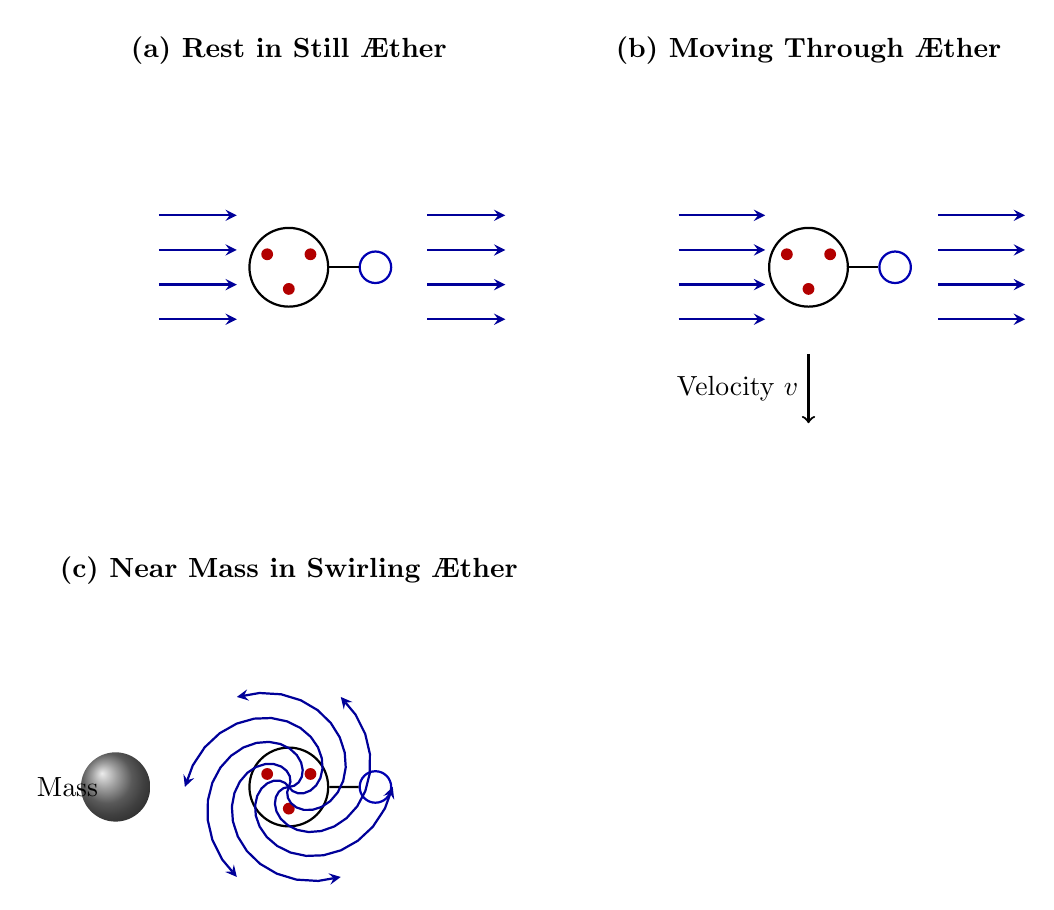
\begin{tikzpicture}[scale=1.1]
        % Styles
        \tikzstyle{proton}=[circle,draw=black,thick,minimum size=1cm]
        \tikzstyle{electron}=[circle,draw=blue!70!black,thick,minimum size=0.4cm]
        \tikzstyle{flow}=[->,>=stealth,thick,blue!60!black]
        \tikzstyle{knot}=[circle,fill=red!70!black,minimum size=0.15cm,inner sep=0pt]

        % Case 1: Rest in deep space
        \node at (0,2.5) {\textbf{(a) Rest in Still Æther}};
        \node[proton] (p1) at (0,0) {};
        \node[knot] at (-0.25,0.15) {};
        \node[knot] at (0.25,0.15) {};
        \node[knot] at (0,-0.25) {};
        \node[electron] (e1) at (1,0) {};
        \draw[thick] (p1) -- (e1);
        \foreach \y in {-0.6,-0.2,0.2,0.6}{
            \draw[flow] (-1.5,\y) -- (-0.6,\y);
            \draw[flow] (1.6,\y) -- (2.5,\y);
        }

        % Case 2: Moving through Æther (SR)
        \node at (6,2.5) {\textbf{(b) Moving Through Æther}};
        \node[proton] (p2) at (6,0) {};
        \node[knot] at (5.75,0.15) {};
        \node[knot] at (6.25,0.15) {};
        \node[knot] at (6,-0.25) {};
        \node[electron] (e2) at (7,0) {};
        \draw[thick] (p2) -- (e2);
        \foreach \y in {-0.6,-0.2,0.2,0.6}{
            \draw[flow] (4.5,\y) -- (5.5,\y);
            \draw[flow] (7.5,\y) -- (8.5,\y);
        }
        \draw[->,thick,black] (6,-1) -- (6,-1.8) node[midway,left]{Velocity $v$};

        % Case 3: Near massive body (GR)
        \node at (0,-3.5) {\textbf{(c) Near Mass in Swirling Æther}};
        \node[proton] (p3) at (0,-6) {};
        \node[knot] at (-0.25,-5.85) {};
        \node[knot] at (0.25,-5.85) {};
        \node[knot] at (0,-6.25) {};
        \node[electron] (e3) at (1,-6) {};
        \draw[thick] (p3) -- (e3);
        % Swirling flow lines
        \foreach \a in {0,60,120,180,240,300}{
            \draw[flow,domain=0:1.2,samples=20,variable=\r]
            plot ({\r*cos(\a+200*\r)}, {-6+\r*sin(\a+200*\r)});
        }

        % Mass representation
        \shade[ball color=gray] (-2,-6) circle (0.4) node[left=0.1cm]{Mass};

    \end{tikzpicture}
    \caption{Hydrogen atoms in three conditions: (a) Rest in still Æther; (b) Moving through Æther (SR time dilation); (c) Near a massive body in swirling Æther (GR time dilation). Protons contain three quark knots; electrons shown as bound unknots. Æther flow lines are straight in (a) and (b), curved in (c).}
    \label{fig:hydrogen_time_dilation}
\end{figure}

\section*{6. Possible Tests of the Model}

Any model can be made to fit known data if you’re clever enough with the equations. The real question is: can it predict something new — something that standard theory doesn’t expect — and can we actually check it?

\subsection*{6.1 Laboratory-Scale Experiments}

One of the reasons I’ve focused on the superfluid analogy is that, in principle, we can build small versions of the system in the lab. A Bose–Einstein condensate (BEC) is the natural candidate.

If we could produce a stable, single vortex in a BEC and embed a “clock” — some repeatable quantum or optical process — at a controlled radius from the core, the model predicts a measurable slowing of that process compared to a reference clock outside the vortex field.

The challenges are obvious:
\begin{itemize}
    \item The slowing would be tiny at achievable swirl velocities.
    \item The clock would need extraordinary precision.
    \item Isolating the effect from noise would be non-trivial.
\end{itemize}

Still, even a null result at high precision would be valuable — it would constrain the possible parameter space of the Æther model.

\subsection*{6.2 Astrophysical Clues}

If the Æther is real and vorticity can mimic gravitational time dilation, then regions with intense rotational flow — such as around rapidly spinning neutron stars — might show subtle deviations from general relativity’s predictions.

For example, the model might produce slightly different pulse arrival times for signals from pulsars skimming the edge of such regions, especially if the swirl profile departs from the “escape-velocity” form required to match Schwarzschild exactly.

\subsection*{6.3 The “Small Difference, Big Stakes” Principle}

I should stress that I’m not expecting the model to overthrow relativity wholesale. That would be naive. Instead, the aim is to find situations where the two pictures agree \textit{almost} perfectly — but not quite. Those small mismatches are where discovery happens.

The first detection of gravitational waves didn’t come from finding a big, glaring violation of Newtonian gravity; it came from measuring tiny distortions in spacetime and confirming they matched the waveforms predicted by relativity. The same principle applies here.

\subsection{Physical Interpretation}

In both the SR and GR analogues, the slowing of time is the slowing of all oscillatory processes within the atom's knotted-field structure. The hydrogen atom's ``clock'' --- set by the frequencies of its internal interactions --- ticks more slowly when part of the Æther's propagation capacity is already committed to bulk motion or swirl. To the atom itself, all processes remain internally consistent; the difference appears only in comparison with a reference clock in still Æther.

\section{Discussion and Conclusion}

The VAM interpretation of time dilation offers a unified mechanical picture: both velocity-based (special relativistic) and gravity-based (general relativistic) time dilation emerge from the same root cause --- the motion of the Æther relative to the local matter system. In this framework, the quark and electron knots forming an atom are not abstract quantum objects in a static spacetime, but dynamic topological features embedded in a moving fluid medium.

This approach maintains mathematical agreement with the Lorentz factor and the gravitational redshift formula, ensuring consistency with observed relativistic phenomena, while replacing the geometric interpretation of spacetime with a kinetic one. The Æther's flow state, whether translational or vortical, directly regulates the rate at which physical processes occur.

Future work should quantify the expected deviations between the VAM predictions and those of general relativity in scenarios where the Æther swirl profile departs from the exact escape-velocity form. Laboratory analogues using superfluids or Bose–Einstein condensates may offer a route to experimental tests. Astrophysical observations, particularly in regions of intense vorticity such as near rotating neutron stars, could provide further constraints or validation.

In summary, VAM reframes time dilation not as an abstract geometric effect, but as a tangible consequence of motion in a physical medium, linking the behavior of fundamental particles directly to the state of the cosmic fluid in which they are immersed.


\end{document}